\documentclass[tikz,border=10pt]{standalone}
\usepackage{tikz}

\begin{document}

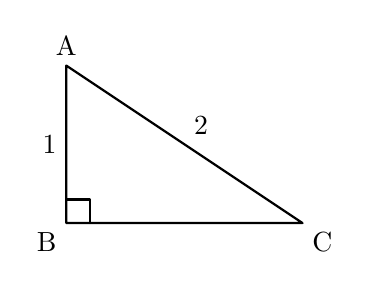
\begin{tikzpicture}[scale=1, line cap=round, line join=round]

% Define coordinates
% Coordinates are adjusted slightly to maintain visibility at scale 1
\coordinate (B) at (0,0);
\coordinate (A) at (0,2);
\coordinate (C) at (3,0);

% Draw the triangle segments
\draw[thick] (A) -- (B) -- (C) -- cycle;

% Draw right angle symbol at B
\draw[thick] (0,0.3) -- (0.3,0.3) -- (0.3,0);

% Add labels for vertices exactly as in the image
\node[above] at (A) {A};
\node[below left] at (B) {B};
\node[below right] at (C) {C};

% Add measurements/labels
\node[left] at (0,1) {1};
\node[above right] at (1.5,1) {2};

\end{tikzpicture}

\end{document}
